% Template:     Informe LaTeX
% Documento:    Archivo de ejemplo
% Versión:      8.3.6 (23/08/2024)
% Codificación: UTF-8
%
% Autor: Pablo Pizarro R.
%        pablo@ppizarror.com
%
% Manual template: [https://latex.ppizarror.com/informe]
% Licencia MIT:    [https://opensource.org/licenses/MIT]

% ------------------------------------------------------------------------------
% NUEVA SECCIÓN
% ------------------------------------------------------------------------------
% Las secciones se inician con \section, si se quiere una sección sin número se
% pueden usar las funciones \sectionanum (sección sin número) o la función
% \sectionanumnoi para crear el mismo título sin numerar y sin aparecer en el índice
\section{Informes con \LaTeX}

% SUB-SECCIÓN
% Las sub-secciones se inician con \subsection, si se quiere una sub-sección
% sin número se pueden usar las funciones \subsectionanum (nuevo subtítulo sin
% numeración) o la función \subsectionanumnoi para crear el mismo subtítulo sin
% numerar y sin aparecer en el índice
\subsection{Una breve introducción}
	
	Este es un párrafo, puede contener múltiples \quotes{Expresiones} así como fórmulas o referencias\footnote{Las referencias se hacen utilizando la expresión \texttt{\textbackslash label}\{etiqueta\}.} como \eqref{eqn:identidad-imposible} o (\ref{img:anexo-2}). A continuación se muestra un ejemplo de inserción de imágenes (como la Figura \ref{img:testimage}) con el comando \href{https://latex.ppizarror.com/informe.html#hlp-imagen}{\textbackslash insertimage}:

	% Esta instrucción, añadida en la v6.5.5 permite cambiar el título de cada
	% objeto en el índice de cada objeto. Este título es solo válido hasta el
	% primer objeto que lo llame, luego este se restablecerá. Por mientras solo
	% se ofrece compatibilidad para las funciones de imágenes. Los entornos como
	% images o sourcecode aún no tienen compatibilidad
	\setindexcaption{Título de la imagen en el índice.}

	% Para insertar una imagen se puede usar la función \insertimage la cual
	% toma un primer parámetro opcional para definir una etiqueta (dentro de
	% los corchetes), luego toma la dirección de la imagen, sus parámetros
	% (en este caso se definió la escala de 0.12) y una leyenda opcional
	\insertimage[\label{img:testimage}]{ejemplos/test-image.png}{scale=0.12}{Where are you? de \quotes{Internet}.}

	A continuación\footnote{Como se puede observar las funciones \texttt{\textbackslash insert...} añaden un párrafo automáticamente.} se muestra un ejemplo de inserción de ecuaciones simples con el comando \href{https://latex.ppizarror.com/informe.html#hlp-formulae}{\textbackslash insertequation}:

	% Se inserta una ecuación, el primer parámetro entre [] es opcional
	% (permite identificar con una etiqueta para poder referenciarlo después
	% con \ref), seguido de aquello se escribe la ecuación en modo bruto sin signos $
	\insertequation[\label{eqn:identidad-imposible}]{\pow{a}{k}=\pow{b}{k}+\pow{c}{k} \quad \forall k>2}

	% Notar que no se requiere añadir un salto de línea después de insertar una imagen
	Este template \cite{template} ha sido diseñado para que sea completamente compatible con editores \LaTeX\ para escritorio y de manera online\scite{overleaf}. La compilación es realizada siempre usando las últimas versiones de las librerías, además se incluyen los parches oficiales para corregir eventuales \textit{warnings}. \\

	Este es un nuevo párrafo. Para crear uno basta con usar \textbackslash\textbackslash\ en el anterior, lo que fuerza una nueva línea. También se pueden insertar con el comando \texttt{\textbackslash newp} si el compilador de latex arroja una alerta del tipo \textit{Underfull \textbackslash hbox (badness 10000) in paragraph at lines ...}

% SUB-SECCIÓN
\subsection{Añadiendo tablas}

	También puedes usar tablas, ¡Crearlas es muy fácil!. Puedes usar el plugin \href{https://www.ctan.org/tex-archive/support/excel2latex}{Excel2Latex} \cite{excel2latex} de Excel para convertir las tablas a \LaTeX\ o bien utilizar el \quotes{creador de tablas online} \cite{tablesgenerator}.

	% Tabla generada con el plugin Excel2Latex
	\begin{table}[H]
		\centering
		\caption{Ejemplo de tablas.}
		\begin{tabular}{ccc}
			\hline
			\textbf{Columna 1} & \textbf{Columna 2} & \textbf{Columna 3} \bigstrut\\
			\hline
			$\omega$ & $\nu$ & $\delta$ \bigstrut[t]\\
			$\xi$ & $\kappa$ & $\varpi$ \bigstrut[b] \\
			\hline
		\end{tabular}
		\label{tab:tabla-1}
	\end{table}


% ------------------------------------------------------------------------------
% NUEVA SECCIÓN
% ------------------------------------------------------------------------------



\clearpage
\section{Pregunta 2}
\begin{itemize}
	\item \textbf{Escriba las condiciones necesarias para encontrar una solución óptima, utilizando el principio del máximo.}

Se busca el obtener las condiciones necesarias para encontrar la solucion al problema de optimización, utilizando el principio del máximo o Pontryagin. Para ello, se considera el siguiente problema de optimización:

\begin{align}
	 J = \int_{0}^{T} (ph(t) - cu(t))dt
\end{align}
Donde tanto las condiciones de borde como la dinamica del sistema vienen caracterizadas por:
\begin{align}
	\dot{x}  rx(t) \left(1 - \frac{x(t)}{K}\right) - h(t) = 0\\
	x(0) = x_0
\end{align}
Luego para encontrar la solución óptima, se plantea el Hamiltoniano asociado al problema de optimización:
\begin{align}
	H(x,u,t,\lambda) = ph(t) - cu(t) + \lambda \left( rx(t) \left(1 - \frac{x(t)}{K}\right) - h(t) \right)
\end{align}
Dado que $h(t)=x(t)u(t)$ reemplazando sobre lo anterior temenos que el Hamiltoniano sera tal que:
\begin{align}
	H(x,u,t,\lambda) = px(t)u(t) - cu(t) + \lambda \left( rx(t) \left(1 - \frac{x(t)}{K}\right) - x(t)u(t) \right)
\end{align}
Donde los $\lambda$ son los multiplicadores de Lagrange asociados a las restricciones del problema. Luego, se plantean las condiciones de optimalidad asociadas al principio del máximo.
\begin{align}
	\dot{\lambda}&= -\frac{\partial H}{\partial x}\\ 
	             &= -\frac{\partial}{\partial x} \left( px(t)u(t) - cu(t) + \lambda \left( rx(t) \left(1 - \frac{x(t)}{K}\right) - x(t)u(t) \right) \right)\\
				 &= -(pqu(t) + \left(r - \frac{2rx(t)}{K}\right)-qu(t))\lambda) 
\end{align}
Ademas debemos considerar que x(T) es una variable libre dado el enunciado, por lo que tendremos que:
\begin{align}
	\lambda(T) = 0 
\end{align}
Por lo que se obtiene una condicion terminal. Finalmente para el analisis de la entrada tenemos que considerar que esta puede tomar dos valores, por lo que factorizando el Hamiltoniano en función de u(t) se obtiene que:
\begin{align}
    H = \lambda r x(t) \left( 1 - \frac{x}{K} \right) + u(t) \left( q x(t) (p - \lambda) - c \right)
\end{align}
Vemos por tanto que u(t) es una funcion lineal al hamiltoniano por lo que podemos definir dos condiciones tal que:
\begin{align*}
    u^*(t) &= 0 \quad \text{cuando} \quad q x(t) (p - \lambda(t)) - c < 0 \\
    u^*(t) &= E \quad \text{cuando} \quad q x(t) (p - \lambda(t)) - c > 0
\end{align*}
Por lo que separando por casos se tendra que:
\begin{align}
    \text{Para } u \equiv 0 \text{ tenemos:} \quad
    \begin{cases}
        \dot{x} = r x \left(1 - \frac{x}{K}\right) \\
        \dot{\lambda} = -r \left(1 - \frac{2x}{K}\right) \lambda
    \end{cases}
\end{align}

\begin{align}
    \text{Para } u \equiv E \text{ tenemos:} \quad
    \begin{cases}
        \dot{x} = r x \left(1 - \frac{x}{K}\right) - q x E \\
        \dot{\lambda} = -(p q E + \left(r \left(1 - \frac{2x}{K}\right) - q E\right)\lambda)
    \end{cases}
\end{align}
De esta manera se tiene que el comportamiento de la solución óptima se encuentrara determinada por los diferentes casos de u(t) que se puede caracterizar mediante:
\begin{align}
	F(x),\lambda)= qx(t)(p-\lambda) -c
\end{align}
Donde si es esta es mayor a 0 , se encontrara se tendra que u*(t) = E, mientras que si es menor a 0 se tendra que u*(t) = 0.
	\item \textbf{Simule curvas de nivel en el plano (x, $\phi$), con $\phi$ el coestado. Interprete los resultados y concluya sobre el comportamiento óptimo de u(t).}\\
Se busca obtener las curvas de nivel en el plano (x, $\lambda$) para esto se hace uso de \textit{Matlab} tal que permita resolver las ecuaciones diferenciales asociadas a las condiciones de optimalidad obtenidas en el punto anterior para los diferentes casos, dando como resultado lo siguiente:
\begin{figure}[H]
	\centering
	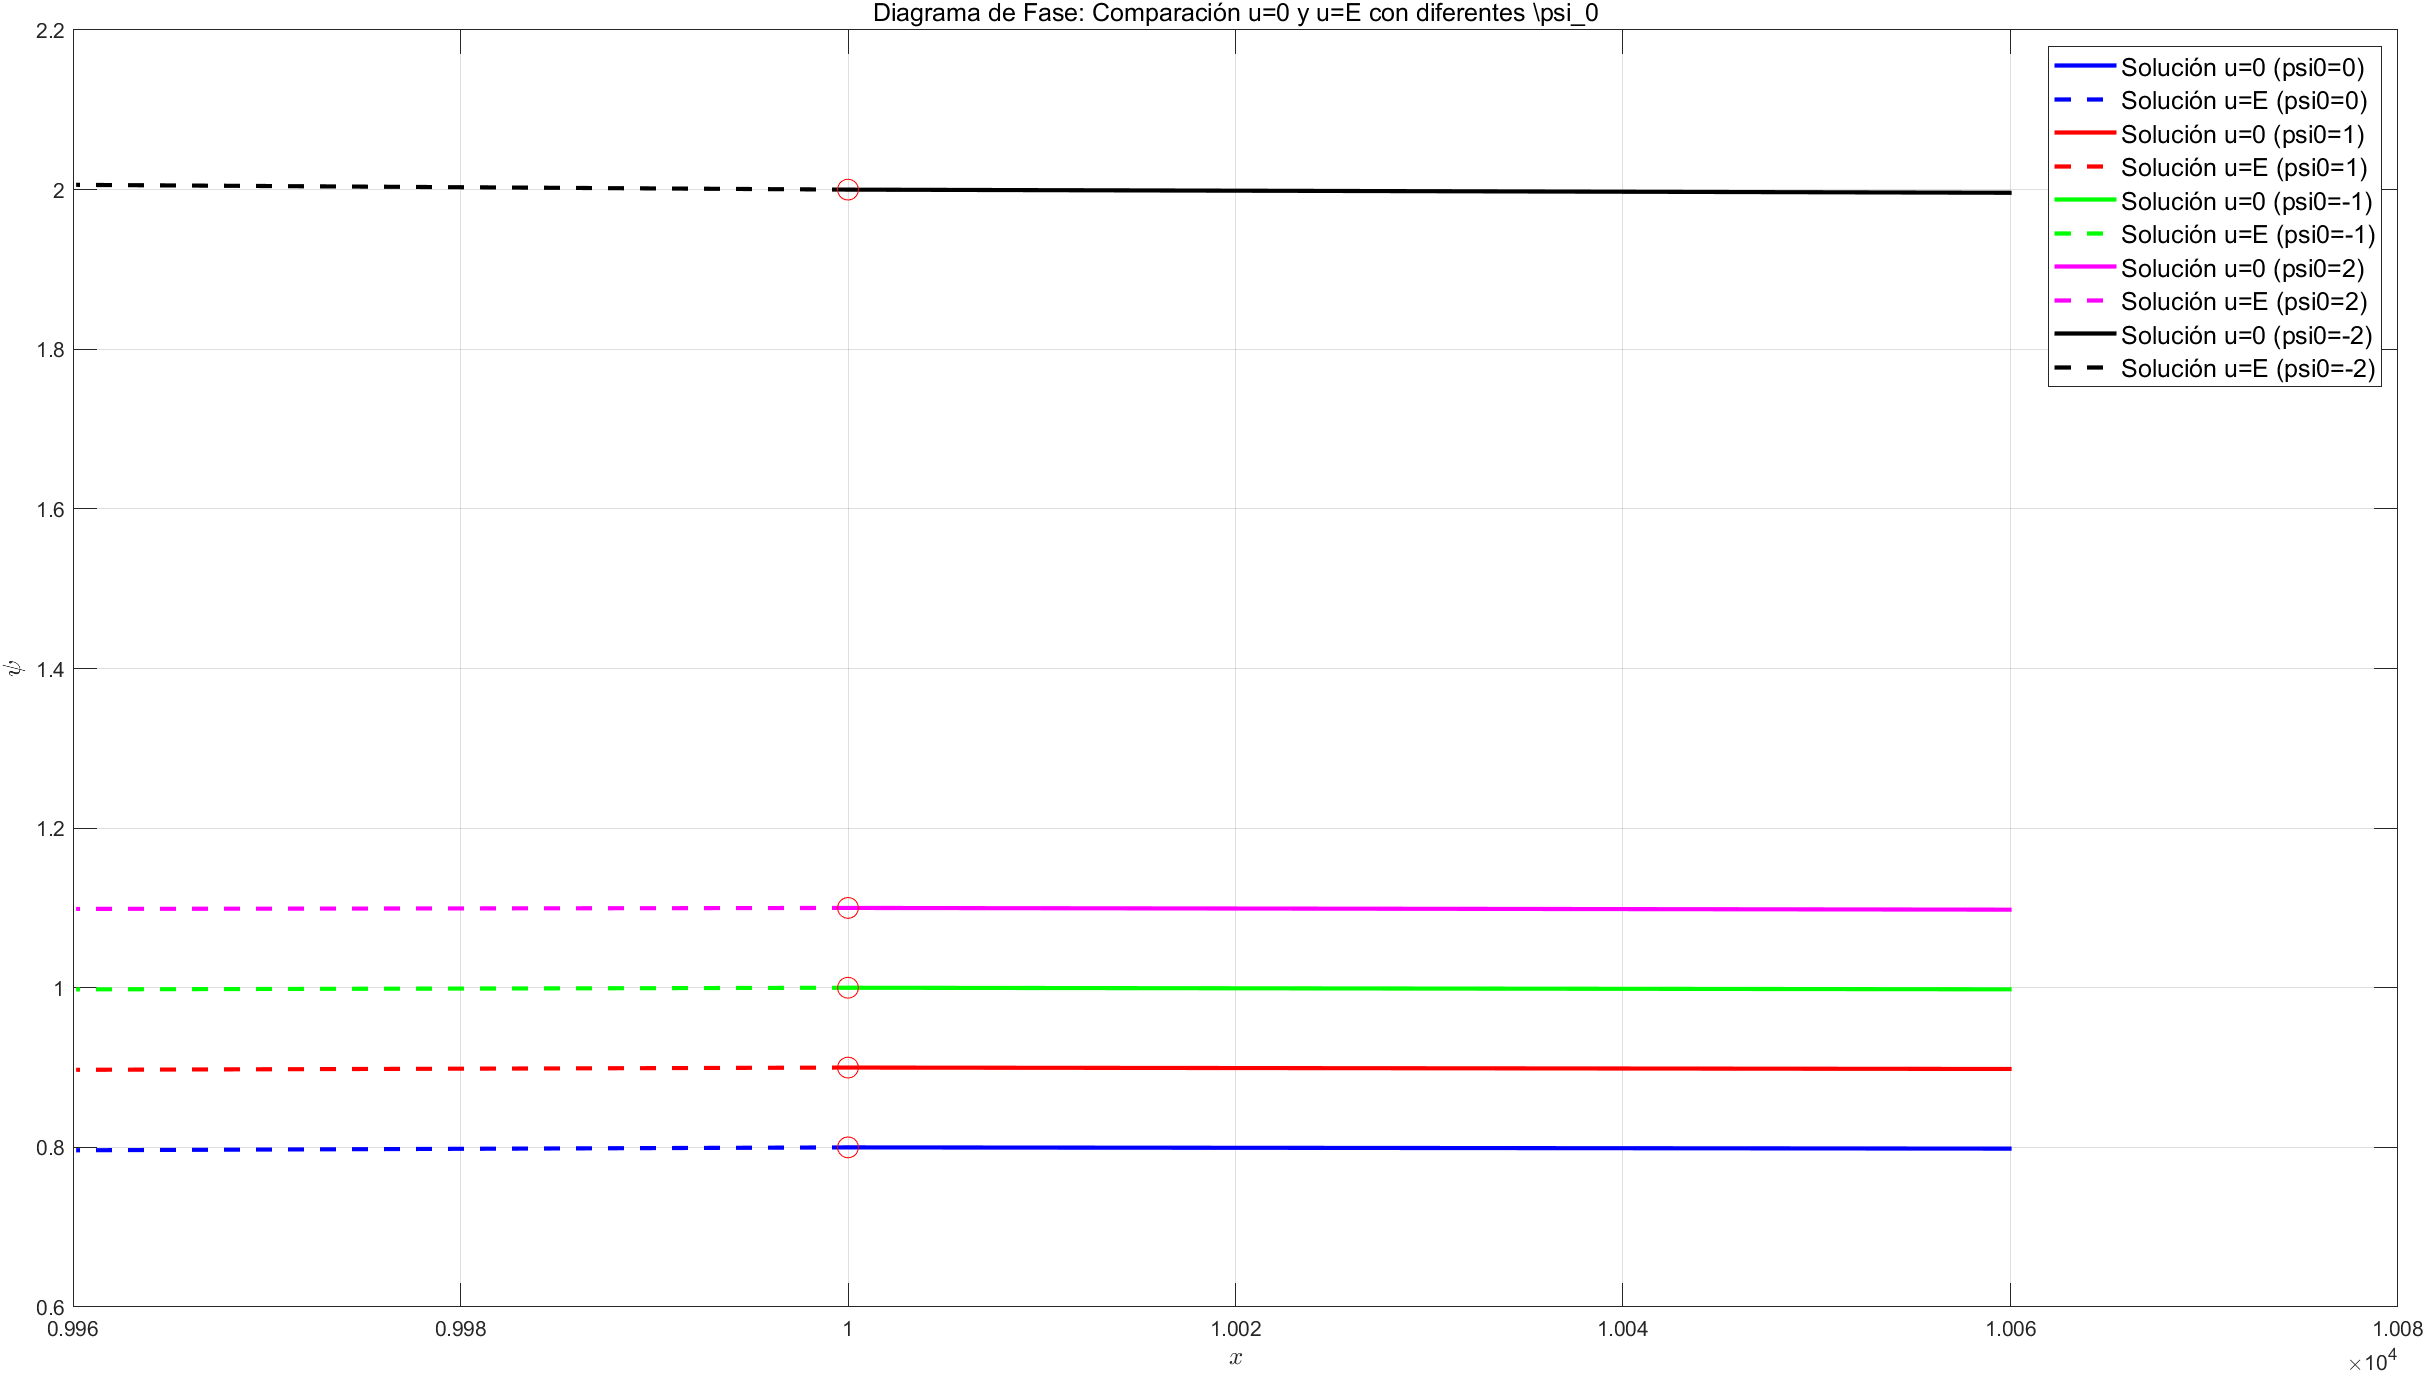
\includegraphics[width=0.9\textwidth]{img/[P2] Curvas de nivel.png}
	\caption{Curvas de nivel en el plano (x, $\lambda$) tanto para $u=0$ como para $u=E$ para los diferentes valores de $\lambda_{0}$, en particular $\lambda_{0} = \{0.8, 0.9, 1, 1.1, 2\}$.}
	\label{img:curvas-nivel}
\end{figure}
Podemos analizar algunos valores de $\lambda_0$ en particular para obtener una mejor interpretacion del grafico con lo que se obtiene que:
\begin{figure}[H]
	\centering
	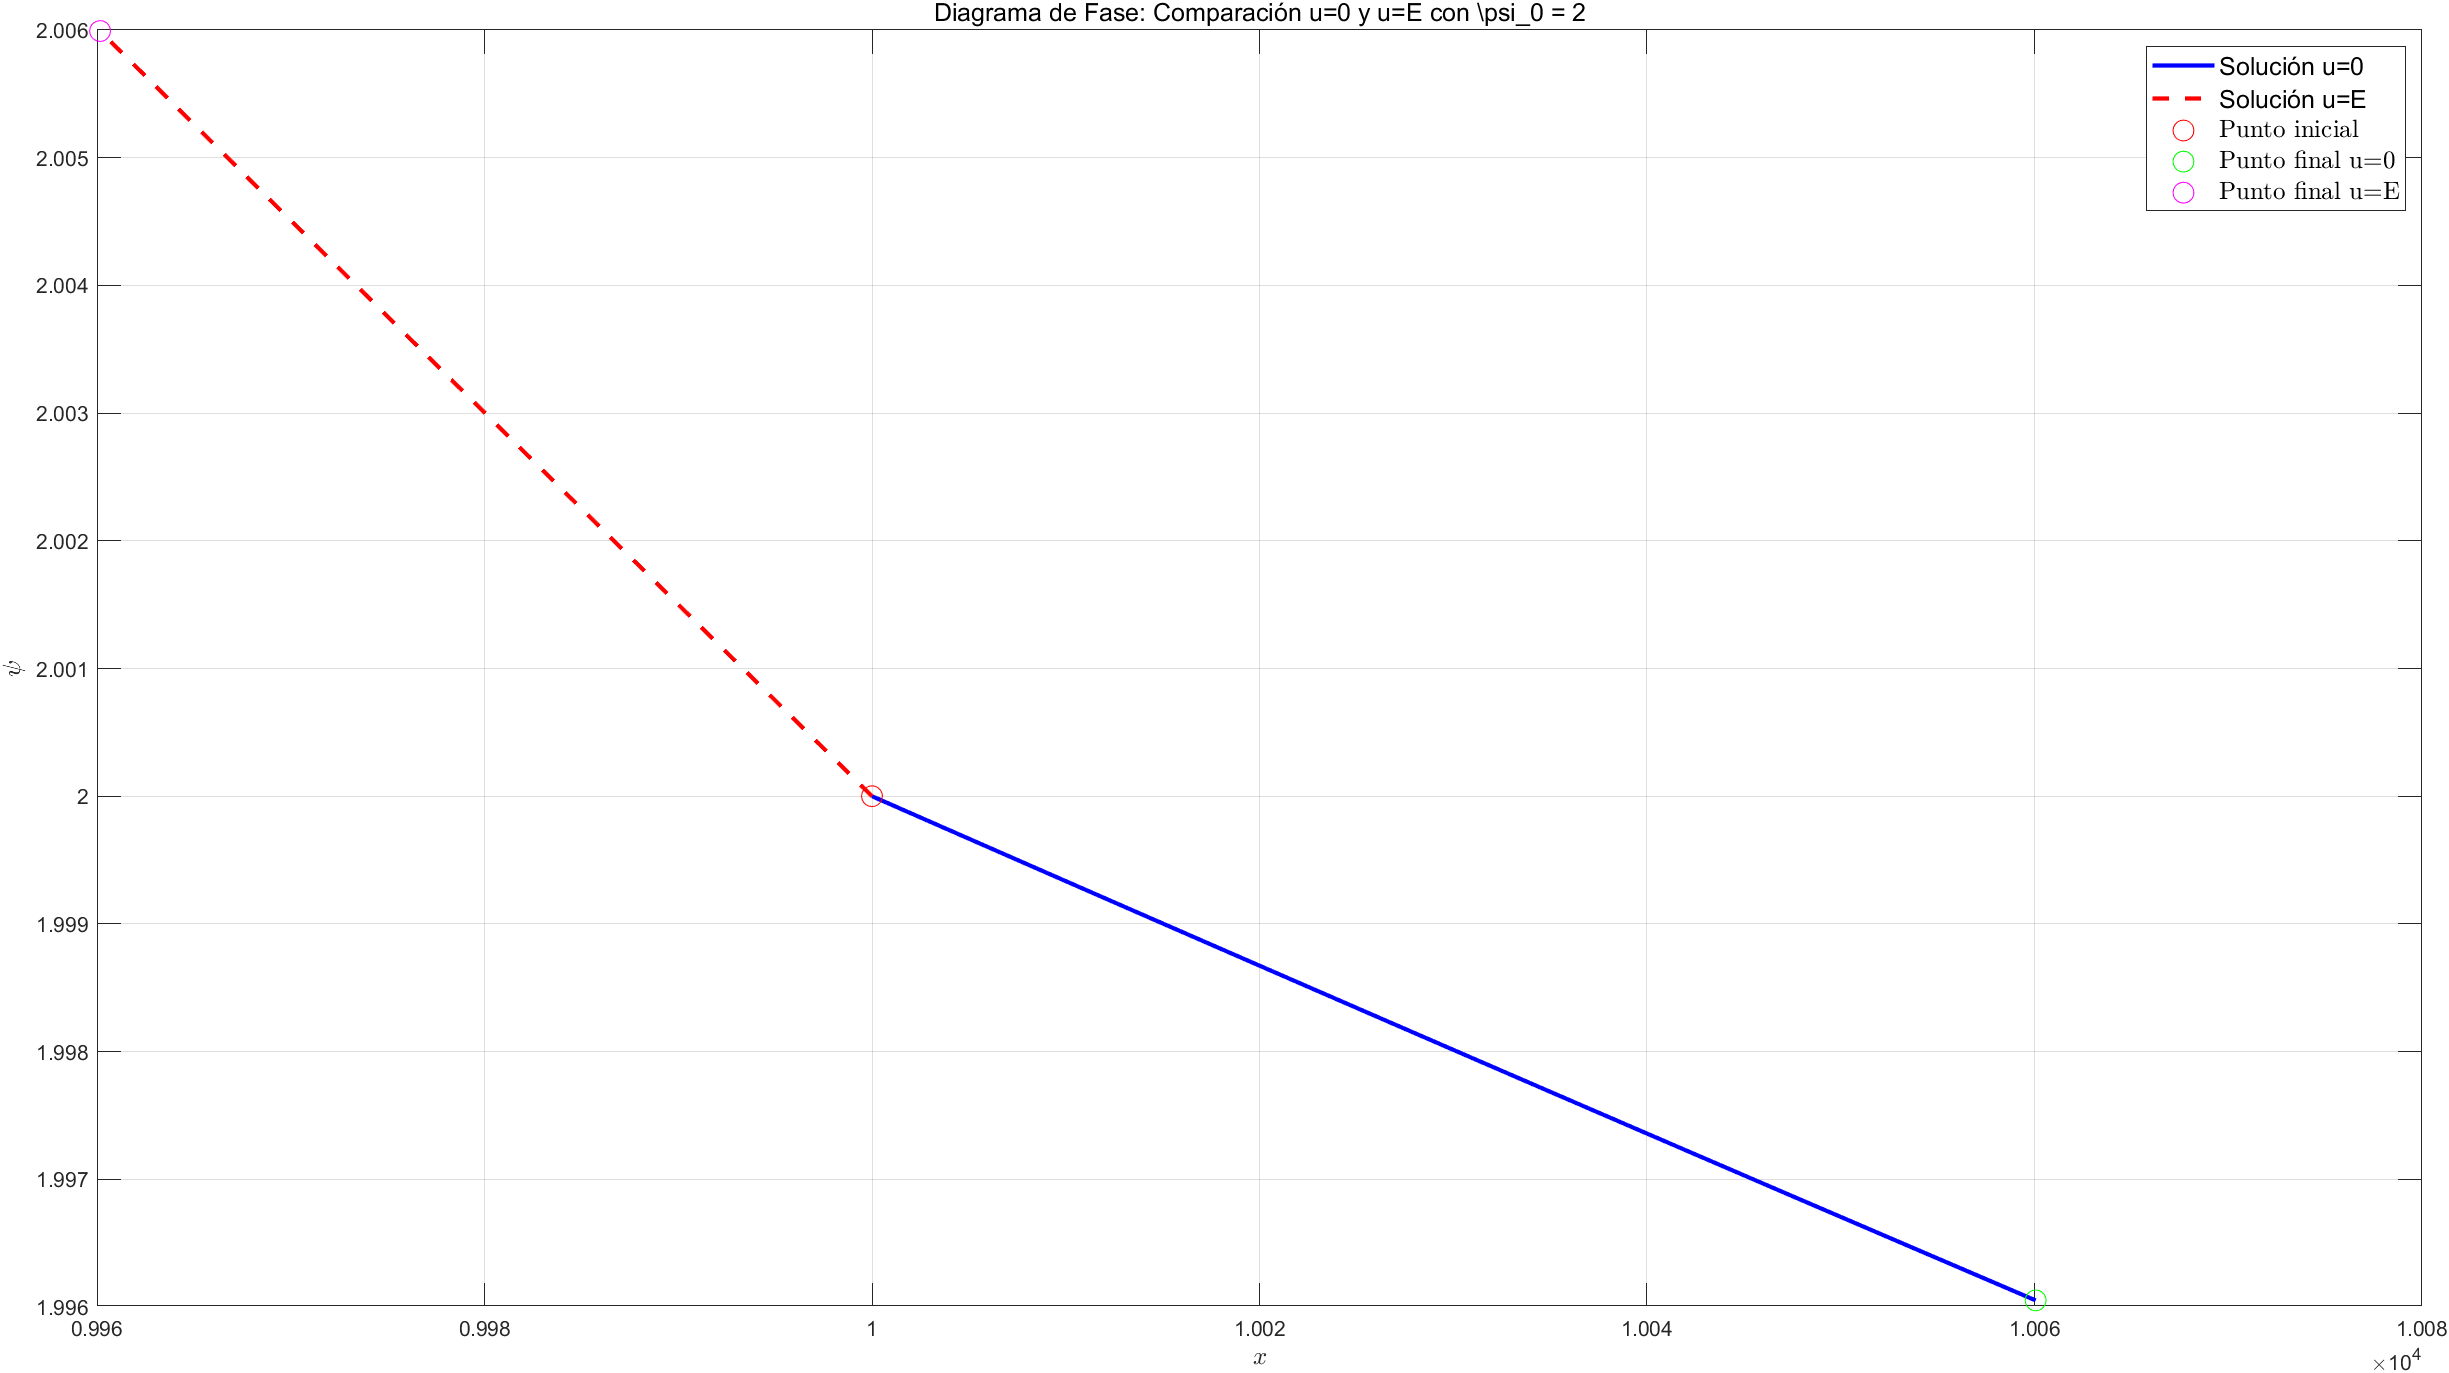
\includegraphics[width=0.9\textwidth]{img/[P2] Phi 2.png}
	\caption{Curvas de nivel en el plano (x, $\lambda$) tanto para $u=0$ como para $u=E$ para $\lambda_{0}=2$.}
	\label{img:curvas-nivel}
\end{figure}
\begin{figure}[H]
	\centering
	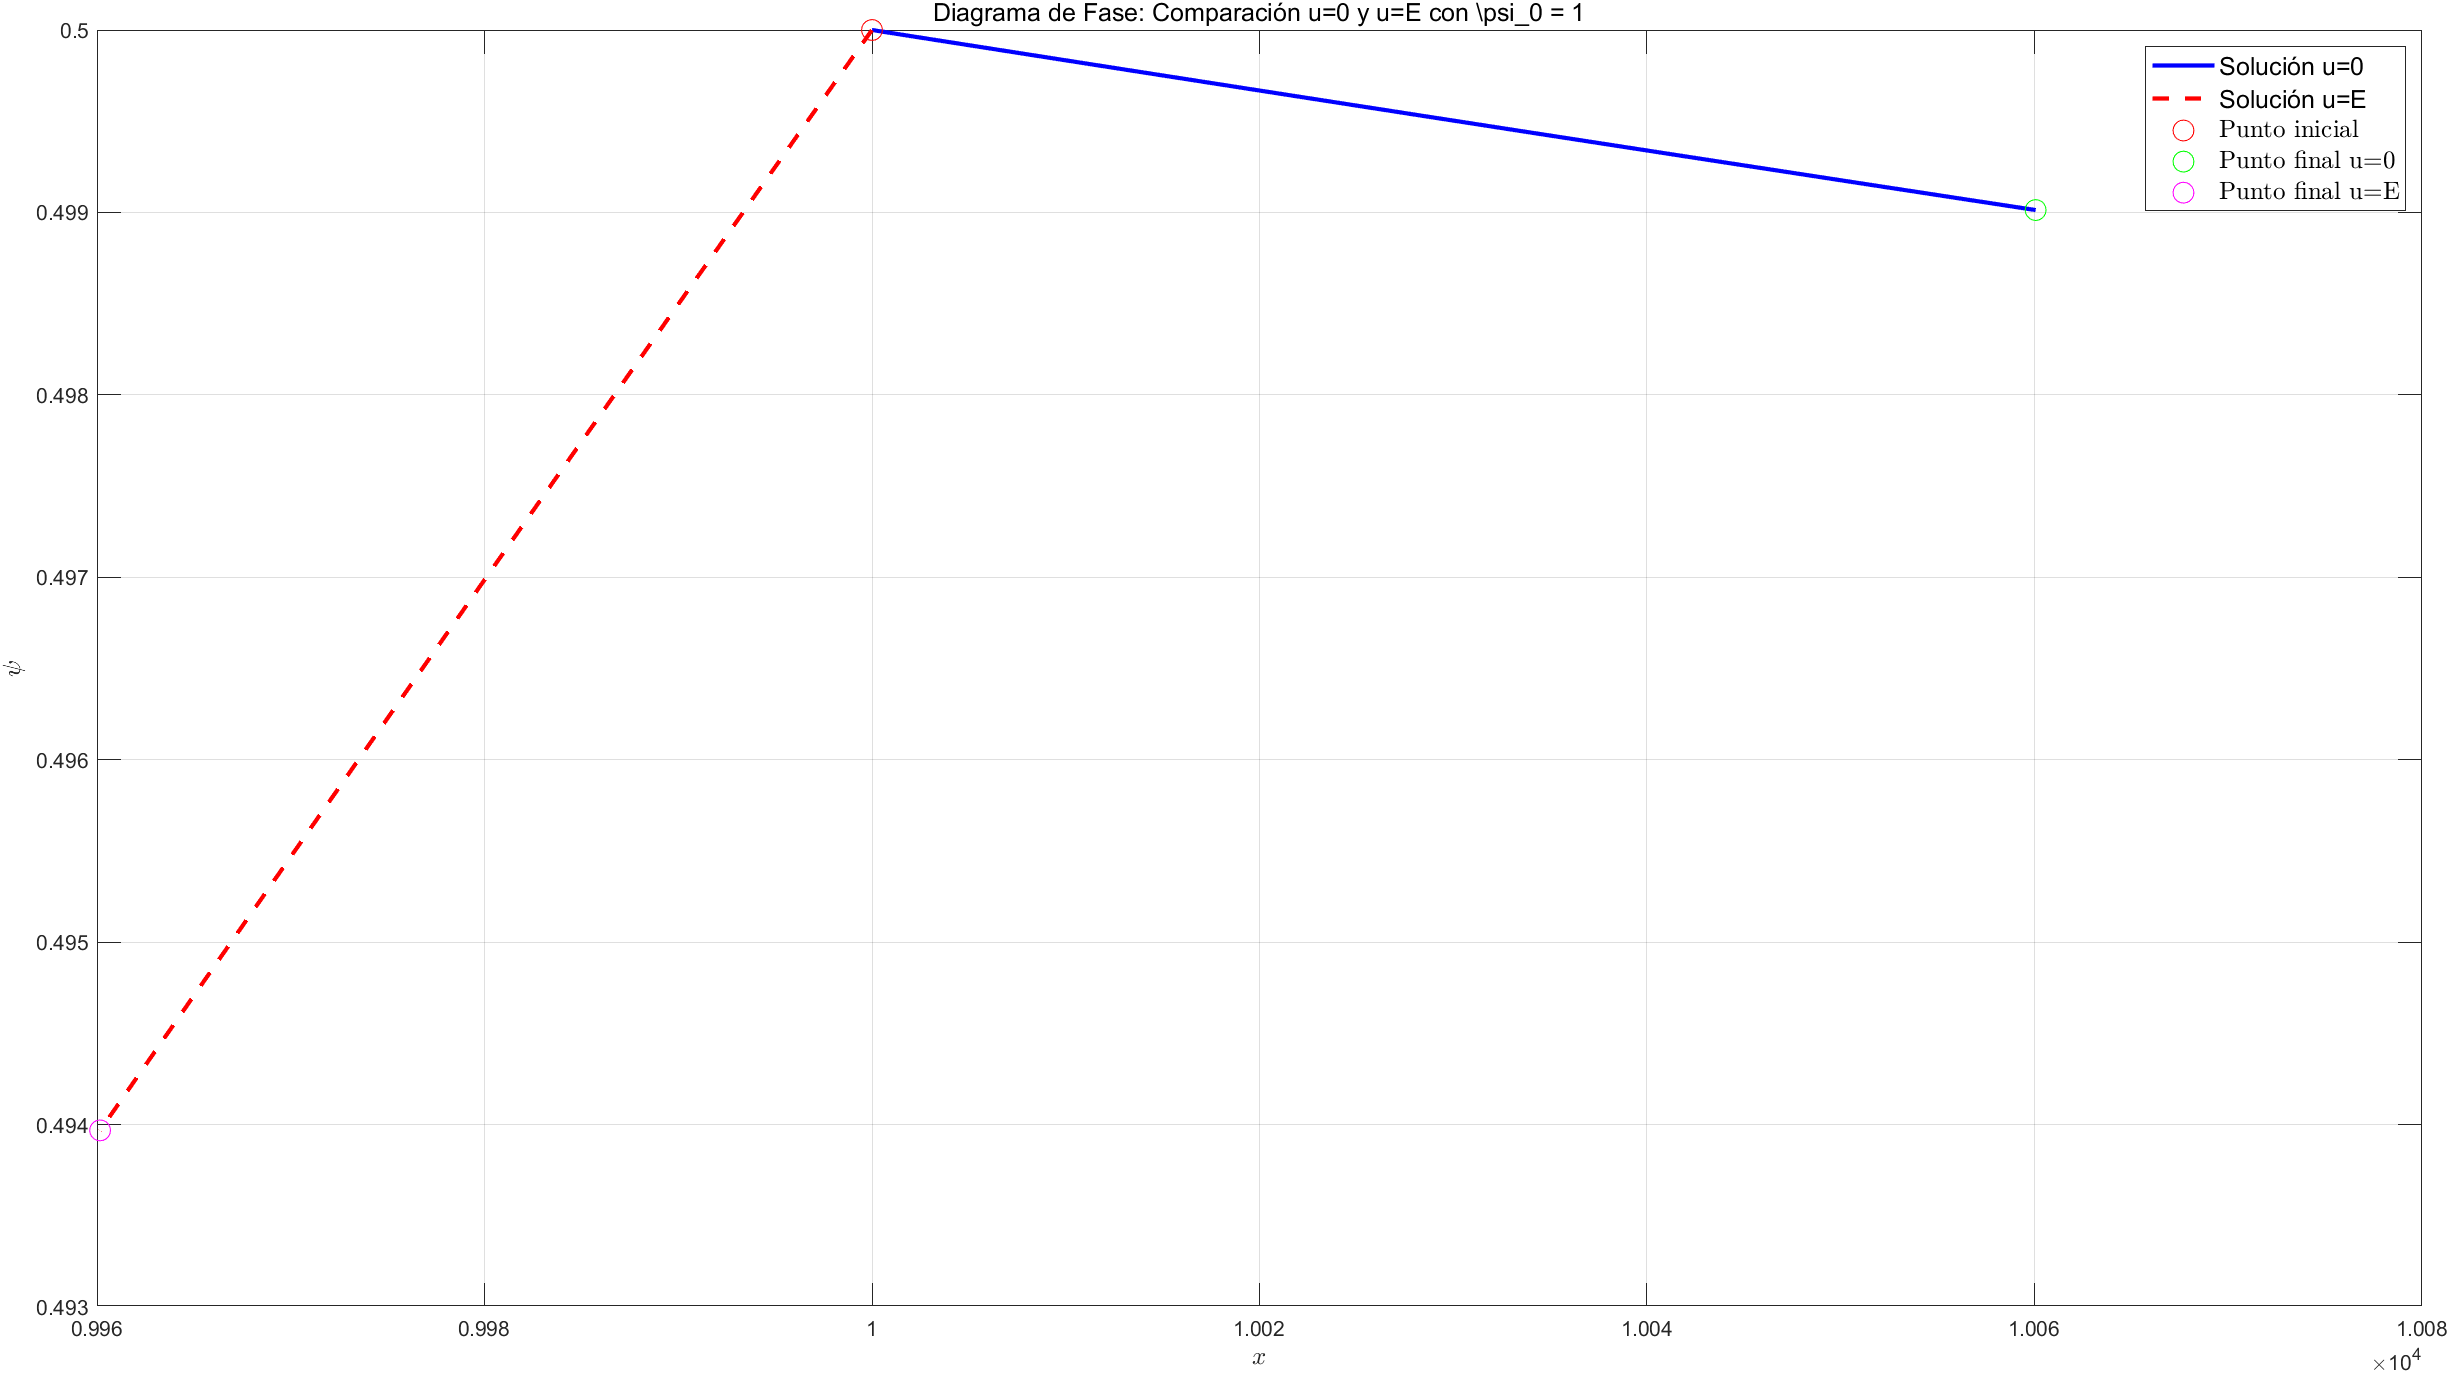
\includegraphics[width=0.9\textwidth]{img/[P2] Phi 0.5.png}
	\caption{Curvas de nivel en el plano (x, $\lambda$) tanto para $u=0$ como para $u=E$ para $\lambda_{0}=0.5$.}
	\label{img:curvas-nivel}
\end{figure}
Luego se puede observar que el comportamiento de la solución óptima se encuentra determinada por los diferentes casos de u(t) ademas de el valor de la condicion inicial $\lambda_0$.
	\item \textbf{Encuentre una expresión para la acción de control óptima $u^{∗}(t)$ y la dinámica de la
	población de peces resultante $x^{*}(t)$, en función de las constantes conocidas. Grafique e interprete los
	resultados.}\\
Dado que se busca obtener una expresion para el control optimo $u^{*}(t)$ y la dinamica de la poblacion de peces resultante $x^{*}(t)$, se debe tener en cuenta el tiempo para $t_{cambio}$ para el cual se produce el cambio de comportamiento de la solución óptima, debido a que es importante saber cuando se produce el cambio de comportamiento en base a las ecuaciones, es por esto que se retoma la funcion $F(x,\lambda)$ obtenida con anterioridad, que nos determina el comportamiento de u(t), se analizara su dinamica en el tiempo para saber cuando esta experimenta un cambio de signo y dado que $\lambda_{0}$ es un parametro de eleccion libre, veremos su comportamiento cuando sea 0.5 y 2. por lo que tomando el primero se tendra que:
\begin{align}
	F(x(0),\lambda(0))&= qx(0)(p-\lambda(0)) -c\\
	      		&= 0.01(10.000)(1-0.5)-0.1\\
				&= 0.05
\end{align}
Por lo que en tal caso dado que F(x(0),$\lambda$(0)) > 0 se tendra que u(t) = E, por lo que se tendra que utilizar el set de ecuaciones asociadas a este caso. Dando al siguiente dinamica:
\begin{figure}
	\centering
	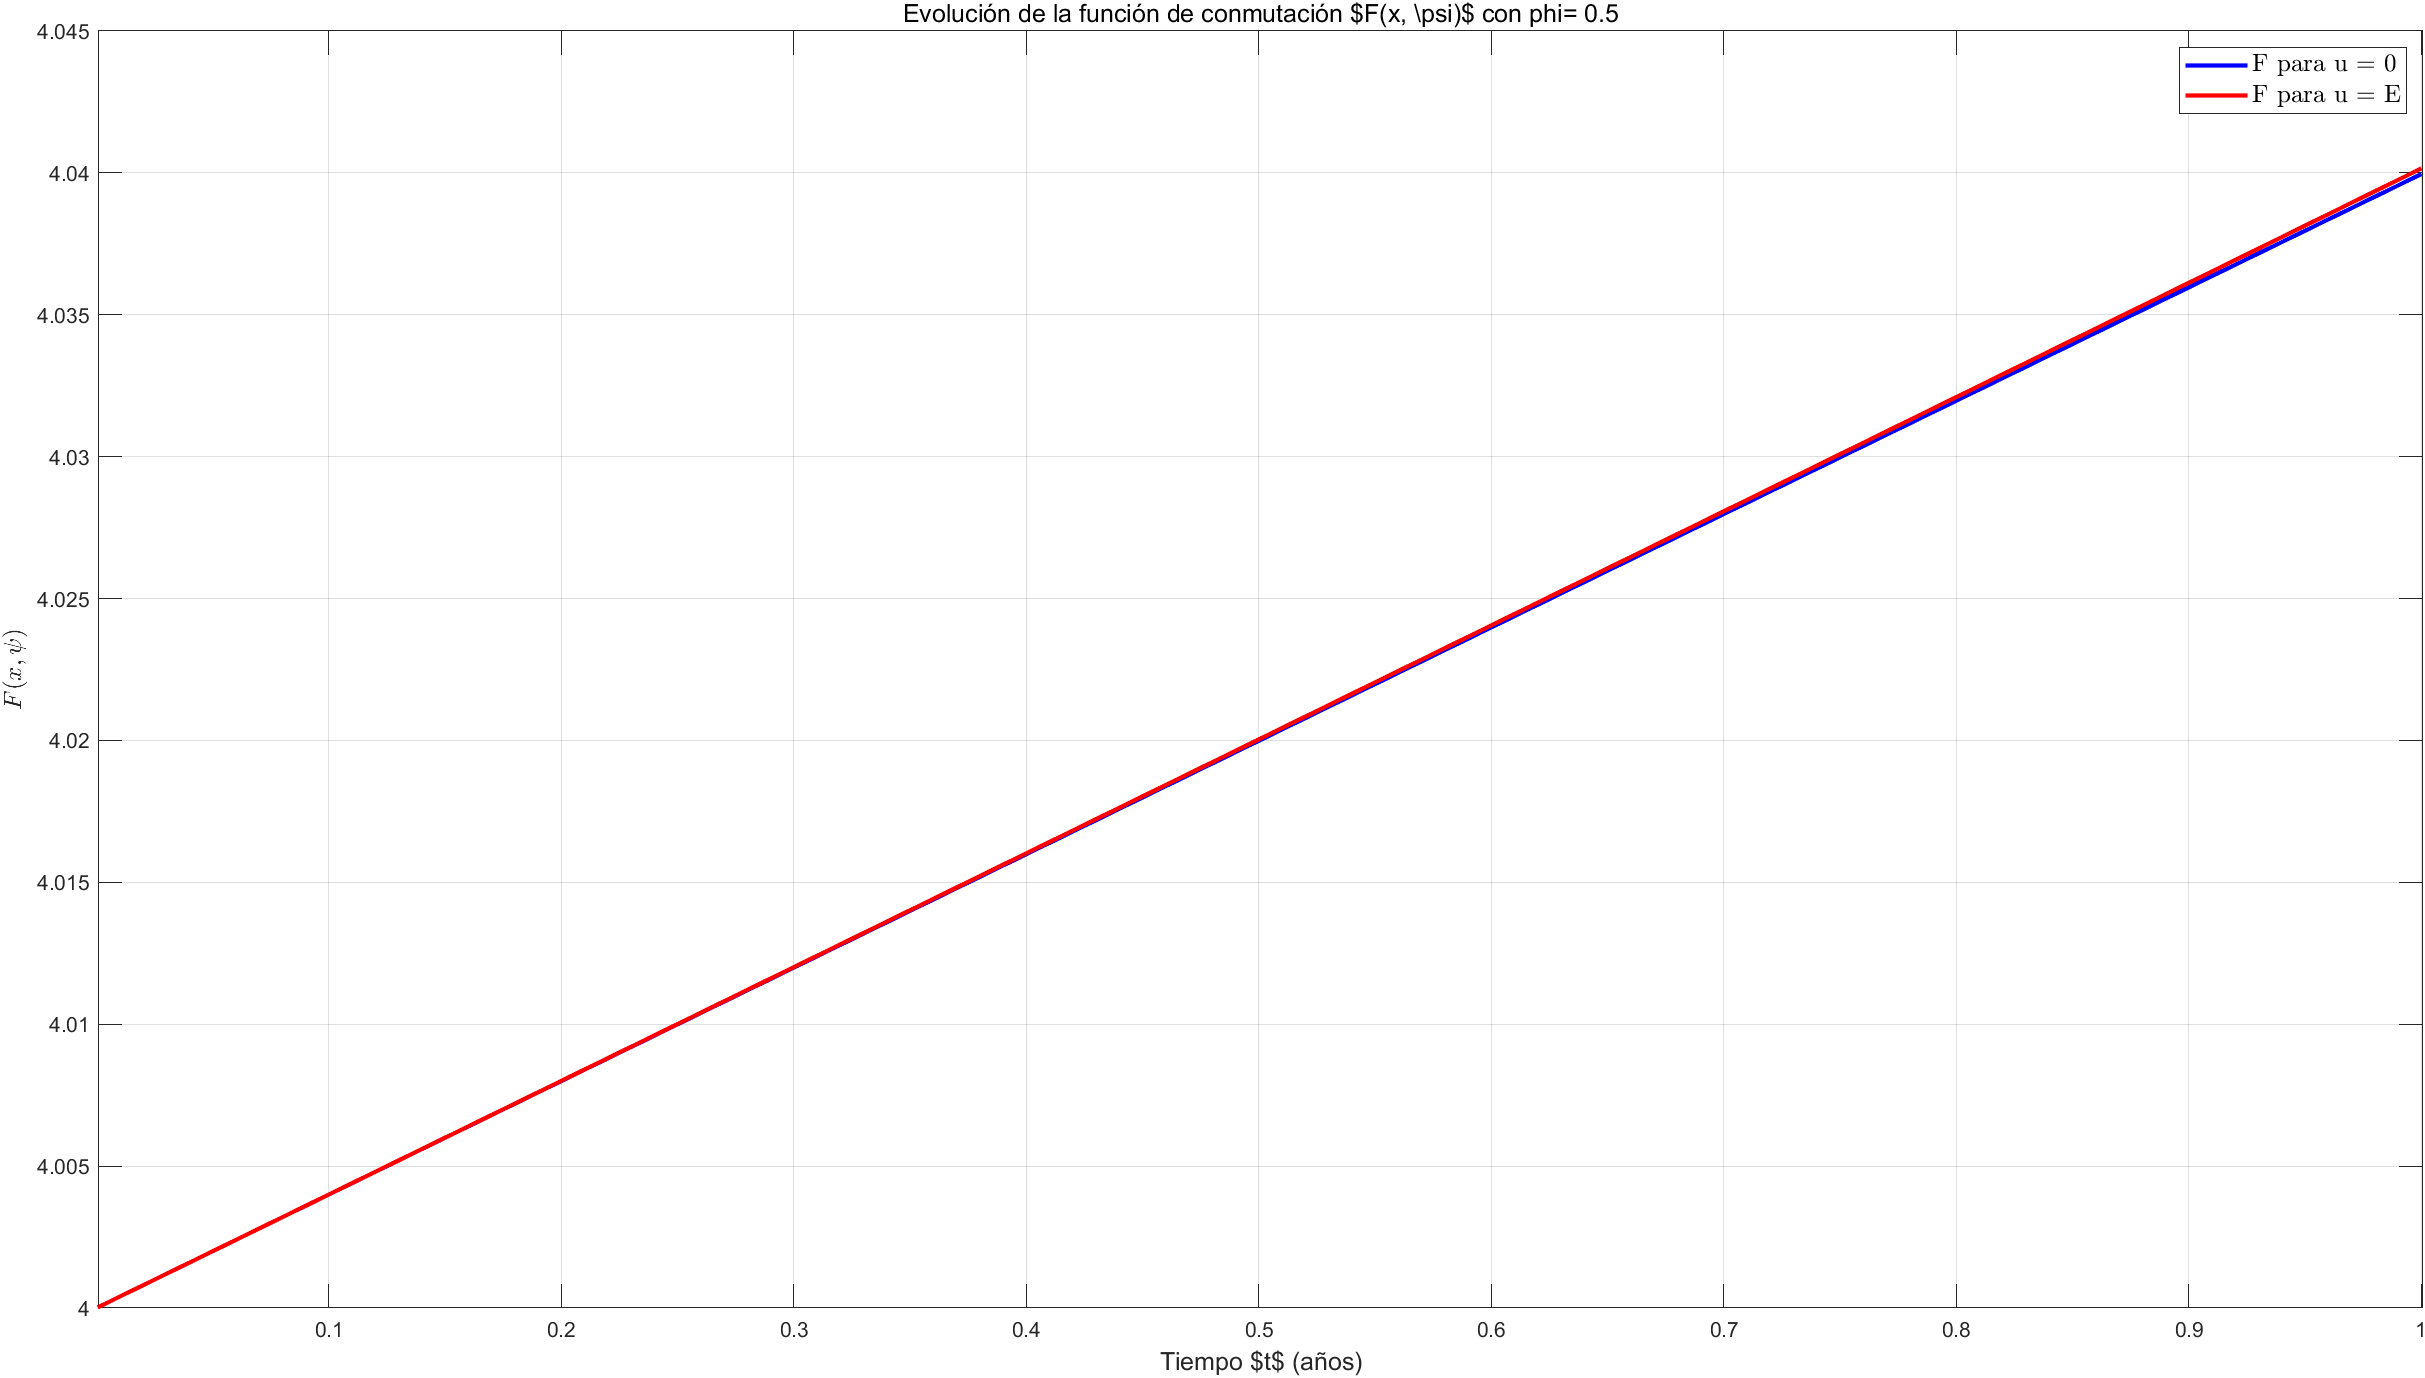
\includegraphics[width=0.9\textwidth]{img/[P2] Phi =0.5.png}
	\caption{Comportamiento de la Dinamica de F(x,$\lambda$) para $\lambda_{0}=0.5$ a lo largo de 1 año.}
	\label{img:dinamica-0.5}
\end{figure}
Vemos que utilizando tanto $u=0$ como $u=E$ este valor sera creciente y por tanto siempre se mantendra la dinamica asocada a 
\end{itemize}
%-------------------	-----------------------------------------------------------
% SUB-SECCIÓN
% ------------------------------------------------------------------------------
